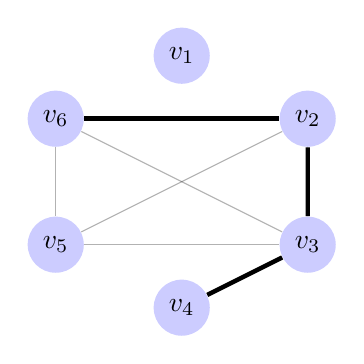
\begin{tikzpicture}
  [scale=.8,auto=left,every node/.style={circle,fill=blue!20}]
  \node (n1) at (2,4) {$v_1$};
  \node (n2) at (4,3)  {$v_2$};
  \node (n3) at (4,1)  {$v_3$};
  \node (n4) at (2,0) {$v_4$};
  \node (n5) at (0,1)  {$v_5$};
  \node (n6) at (0,3)  {$v_6$};

  \foreach \from/\to in {n3/n4,n2/n3, n2/n5, n2/n6, n3/n5, n3/n6, n5/n6}
  \draw[opacity=0.3] (\from) -- (\to);

  \foreach \from/\to in {n6/n2, n2/n3, n3/n4}
  \draw[ultra thick] (\from) -- (\to);

%\draw[ultra thick, red] (n2) -- (n6);
\end{tikzpicture}
